\documentclass[a4paper,12pt]{report}
\usepackage[left=2cm,right=2cm,top=2cm,bottom=3cm]{geometry}

%stuff I've added
\usepackage[utf8]{inputenc}
\usepackage{graphicx}% Include figure files
% \usepackage{dcolumn}% Align table columns on decimal point
% \usepackage{bm}% bold math
\usepackage{acronym}
\usepackage{physics}
% \usepackage{layouts}
\usepackage{acronym}
\usepackage{lipsum} 

\usepackage{amsmath}
\usepackage{amssymb}
\usepackage{svg}
\usepackage{comment}
\usepackage{placeins}
\usepackage{float}
\floatplacement{figure}{H} % the default figure placement specifier

\usepackage{hyperref}
\usepackage{cleveref}
\usepackage{bookmark}

\usepackage{pdfpages} % To be able to include pdfs in the appendix

\usepackage[version=4]{mhchem} % for chemical formulas

\usepackage[style=numeric,
sorting=none,
hyperref=true]{biblatex}
\addbibresource{entire_zotero_library.bib}

% \def\[#1\]{\begin{equation}#1\end{equation}}

% Exrta symbol commands
\newcommand{\tex}[1]{\expval{#1}} %Thermal expectation value
\newcommand{\qex}[1]{\expval{#1}} %Quantum expectation value
\newcommand{\Z}{\mathcal{Z}} %Partition function
\newcommand{\T}{\mathcal{T}} %MCMC Transition function
\newcommand{\A}{\mathcal{A}} %MCMC Acceptance function
\newcommand{\p}{\mathcal{P}} %MCMC Proposal distribution
\newcommand{\nfi}{n^f_i} %FK number operators of f electrons
\newcommand{\nfj}{n^f_j} %FK number operators of f electrons
\newcommand{\s}{\vec{s}} %used to refer to states of the spin system

\usepackage{orcidlink}

%for code blocks
\usepackage{listings}
\usepackage{xcolor}

\definecolor{codegreen}{rgb}{0,0.6,0}
\definecolor{codegray}{rgb}{0.5,0.5,0.5}
\definecolor{codepurple}{rgb}{0.58,0,0.82}
\definecolor{backcolour}{rgb}{0.95,0.95,0.92}
\definecolor{urlblue}{HTML}{007bff}

\lstdefinestyle{mystyle}{
    backgroundcolor=\color{backcolour},   
    commentstyle=\color{codegreen},
    keywordstyle=\color{magenta},
    numberstyle=\tiny\color{codegray},
    stringstyle=\color{codepurple},
    basicstyle=\ttfamily\footnotesize,
    breakatwhitespace=false,         
    breaklines=true,                 
    captionpos=b,                    
    keepspaces=true,                 
    numbers=left,                    
    numbersep=5pt,                  
    showspaces=false,                
    showstringspaces=false,
    showtabs=false,                  
    tabsize=2
}

\lstset{style=mystyle}
%endfor code blocks

% \begin{acronym}
    \newacro{FK}{Falikov-Kimball}
    \newacro{CDW}[CDW]{charge-density wave}
    \newacro{MCMC}{Markov chain Monte Carlo}
    \newacro{ED}{Exact Diagonalisation}
    \newacro{TMM}{Transfer Matrix Methods}
    \newacro{IPR}{Inverse Participation Ratio}
    \newacro{DOS}{density of states}
    \newacro{FTPT}{finite temperature phase transition}
    \newacro{LRI}{Long-Range Ising}
% \end{acronym}

\hypersetup{
    colorlinks = true,
    linkcolor  = black,
    citecolor  = black,
    urlcolor   = urlblue,
}

\urlstyle{same}

\usepackage{wrapfig}
\usepackage{floatflt}

%stuff that came in the template

\usepackage{graphicx}
\usepackage{verbatim}
\usepackage{latexsym}
\usepackage{mathchars}
\usepackage{setspace}

\setlength{\parskip}{\medskipamount}  % a little space before a \par
\setlength{\parindent}{0pt}	      % don't indent first lines of paragraphs
%UHEAD.STY  If this is included after \documentstyle{report}, it adds
% an underlined heading style to the LaTeX report style.
% \pagestyle{uheadings} will put underlined headings at the top
% of each page. The right page headings are the Chapter titles and
% the left page titles are supplied by \def\lefthead{text}.

% Ted Shapin, Dec. 17, 1986

\makeatletter
\def\chapapp2{Chapter}

\def\appendix{\par
 \setcounter{chapter}{0}
 \setcounter{section}{0}
 \def\chapapp2{Appendix}
 \def\@chapapp{Appendix}
 \def\thechapter{\Alph{chapter}}}

\def\ps@uheadings{\let\@mkboth\markboth
% modifications
\def\@oddhead{\protect\underline{\protect\makebox[\textwidth][l]
		{\sl\rightmark\hfill\rm\thepage}}}
\def\@oddfoot{}
\def\@evenfoot{}
\def\@evenhead{\protect\underline{\protect\makebox[\textwidth][l]
		{\rm\thepage\hfill\sl\leftmark}}}
% end of modifications
\def\chaptermark##1{\markboth {\ifnum \c@secnumdepth >\m@ne
 \chapapp2\ \thechapter. \ \fi ##1}{}}%
\def\sectionmark##1{\markright {\ifnum \c@secnumdepth >\z@
   \thesection. \ \fi ##1}}}
\makeatother
%%From: marcel@cs.caltech.edu (Marcel van der Goot)
%%Newsgroups: comp.text.tex
%%Subject: illegal modification of boxit.sty
%%Date: 28 Feb 92 01:10:02 GMT
%%Organization: California Institute of Technology (CS dept)
%%Nntp-Posting-Host: andromeda.cs.caltech.edu
%%
%%
%%Quite some time ago I posted a file boxit.sty; maybe it made it
%%to some archives, although I don't recall submitting it. It defines
%%	\begin{boxit}
%%	...
%%	\end{boxit}
%%to draw a box around `...', where the `...' can contain other
%%environments (e.g., a verbatim environment). Unfortunately, it had
%%a problem: it did not work if you used it in paragraph mode, i.e., it
%%only worked if there was an empty line in front of \begin{boxit}.
%%Luckily, that is easily corrected.
%%
%%HOWEVER, apparently someone noticed the problem, tried to correct it,
%%and then distributed this modified version. That would be fine with me,
%%except that:
%%1. There was no note in the file about this modification, it only has my
%%   name in it.
%%2. The modification is wrong: now it only works if there is *no* empty
%%   line in front of \begin{boxit}. In my opinion this bug is worse than
%%   the original one.
%%
%%In particular, the author of this modification tried to force an empty
%%line by inserting a `\\' in the definition of \Beginboxit. If you have
%%a version of boxit.sty with a `\\', please delete it. If you have my
%%old version of boxit.sty, please also delete it. Below is an improved
%%version.
%%
%%Thanks to Joe Armstrong for drawing my attention to the bug and to the
%%illegal version.
%%
%%                                          Marcel van der Goot
%% .---------------------------------------------------------------
%% | Blauw de viooltjes,                    marcel@cs.caltech.edu
%% |    Rood zijn de rozen;
%% | Een rijm kan gezet
%% |    Met plaksel en dozen.
%% |


% boxit.sty
% version: 27 Feb 1992
%
% Defines a boxit environment, which draws lines around its contents.
% Usage:
%   \begin{boxit}
%	... (text you want to be boxed, can contain other environments)
%   \end{boxit}
%
% The width of the box is the width of the contents.
% The boxit* environment behaves the same, except that the box will be
% at least as wide as a normal paragraph.
%
% The reason for writing it this way (rather than with the \boxit#1 macro
% from the TeXbook), is that now you can box verbatim text, as in
%   \begin{boxit}
%   \begin{verbatim}
%   this better come out in boxed verbatim mode ...
%   \end{verbatim}
%   \end{boxit}
%
%						Marcel van der Goot
%						marcel@cs.caltech.edu
%

\def\Beginboxit
   {\par
    \vbox\bgroup
	   \hrule
	   \hbox\bgroup
		  \vrule \kern1.2pt %
		  \vbox\bgroup\kern1.2pt
   }

\def\Endboxit{%
			      \kern1.2pt
		       \egroup
		  \kern1.2pt\vrule
		\egroup
	   \hrule
	 \egroup
   }	

\newenvironment{boxit}{\Beginboxit}{\Endboxit}
\newenvironment{boxit*}{\Beginboxit\hbox to\hsize{}}{\Endboxit}
\pagestyle{empty}

%

\makeatletter  %to avoid error messages generated by "\@". Makes Latex treat "@" like a letter

% \linespread{1.5} % enable to go back to 1.5 line spacing
\def\submitdate#1{\gdef\@submitdate{#1}}

\def\maketitle{
  \begin{titlepage}{
    %\linespread{1.5}
    \Large Imperial College of Science, Technology and Medicine \\
    %\linebreak
    Department of Physics
    \rm
    \vskip 3in
    \Large \bf \@title \par
  }
  \vskip 0.3in
  \par
  {\Large \@author}
  \vskip 4in
  \par
  Submitted in part fulfilment of the requirements for the degree of 
  \linebreak
  Doctor of Philosophy in Physics of Imperial College of Science, Technology and Medicine \@submitdate
  \vfil
  \end{titlepage}
}

\def\titlepage{
  \newpage
  \centering
  \linespread{1}
  \normalsize
  \vbox to \vsize\bgroup\vbox to 9in\bgroup
}
\def\endtitlepage{
  \par
  \kern 0pt
  \egroup
  \vss
  \egroup
  \cleardoublepage
}

\def\abstract{
  \pagenumbering{arabic}
  \begin{center}{
    \large\bf Abstract}
  \end{center}
  \small
  %\def\baselinestretch{1.5}
  % \linespread{1.5}
  \normalsize
}
\def\endabstract{
  \par
}

\newenvironment{acknowledgements}{
  \cleardoublepage
  \begin{center}{
    \large \bf Acknowledgements}
  \end{center}
  \small
  % \linespread{1.5}
  \normalsize
}{\cleardoublepage}
\def\endacknowledgements{
  \par
}

\newenvironment{dedication}{
  \cleardoublepage
  \begin{center}{
    \large \bf Dedication}
  \end{center}
  \small
  % \linespread{1.5}
  \normalsize
}{\cleardoublepage}
\def\enddedication{
  \par
}

\def\preface{
    % \pagenumbering{roman}
    \pagestyle{plain}
    % \doublespacing
}

\def\body{
    \pagestyle{plain}
    \cleardoublepage    
    \setlength{\parskip}{1.1ex}
    \tableofcontents
    % \cleardoublepage
    % \pagestyle{uheadings}
    % \listoftables
    % \pagestyle{plain}
    % \cleardoublepage

    \listoffigures
    \cleardoublepage

    \pagestyle{fancy}
    \setlength{\parskip}{2ex plus 0.5ex minus 0.2ex}
    \setlength{\parindent}{0pt}
}

\makeatother  %to avoid error messages generated by "\@". Makes Latex treat "@" like a letter

\newcommand{\ipc}{{\sf ipc}}

\newcommand{\Prob}{\bbbp}
\newcommand{\Real}{\bbbr}
% \newcommand{\real}{\Real}
\newcommand{\Int}{\bbbz}
\newcommand{\Nat}{\bbbn}

\newcommand{\NN}{{\sf I\kern-0.14emN}}   % Natural numbers
\newcommand{\ZZ}{{\sf Z\kern-0.45emZ}}   % Integers
\newcommand{\QQQ}{{\sf C\kern-0.48emQ}}   % Rational numbers
\newcommand{\RR}{{\sf I\kern-0.14emR}}   % Real numbers
\newcommand{\KK}{{\cal K}}
\newcommand{\OO}{{\cal O}}
\newcommand{\AAA}{{\bf A}}
\newcommand{\HH}{{\bf H}}
\newcommand{\II}{{\bf I}}
\newcommand{\LL}{{\bf L}}
\newcommand{\PP}{{\bf P}}
\newcommand{\PPprime}{{\bf P'}}
\newcommand{\QQ}{{\bf Q}}
\newcommand{\UU}{{\bf U}}
\newcommand{\UUprime}{{\bf U'}}
\newcommand{\zzero}{{\bf 0}}
\newcommand{\ppi}{\mbox{\boldmath $\pi$}}
\newcommand{\aalph}{\mbox{\boldmath $\alpha$}}
\newcommand{\bb}{{\bf b}}
\newcommand{\ee}{{\bf e}}
\newcommand{\mmu}{\mbox{\boldmath $\mu$}}
\newcommand{\vv}{{\bf v}}
\newcommand{\xx}{{\bf x}}
\newcommand{\yy}{{\bf y}}
\newcommand{\zz}{{\bf z}}
\newcommand{\oomeg}{\mbox{\boldmath $\omega$}}
\newcommand{\res}{{\bf res}}
\newcommand{\cchi}{{\mbox{\raisebox{.4ex}{$\chi$}}}}
%\newcommand{\cchi}{{\cal X}}
%\newcommand{\cchi}{\mbox{\Large $\chi$}}

% Logical operators and symbols
\newcommand{\imply}{\Rightarrow}
\newcommand{\bimply}{\Leftrightarrow}
\newcommand{\union}{\cup}
\newcommand{\intersect}{\cap}
\newcommand{\boolor}{\vee}
\newcommand{\booland}{\wedge}
\newcommand{\boolimply}{\imply}
\newcommand{\boolbimply}{\bimply}
\newcommand{\boolnot}{\neg}
\newcommand{\boolsat}{\!\models}
\newcommand{\boolnsat}{\!\not\models}


% \newcommand{\op}[1]{\mathrm{#1}}
% \newcommand{\s}[1]{\ensuremath{\mathcal #1}}

% Properly styled differentiation and integration operators
\newcommand{\diff}[1]{\mathrm{\frac{d}{d\mathit{#1}}}}
\newcommand{\diffII}[1]{\mathrm{\frac{d^2}{d\mathit{#1}^2}}}
\newcommand{\intg}[4]{\int_{#3}^{#4} #1 \, \mathrm{d}#2}
\newcommand{\intgd}[4]{\int\!\!\!\!\int_{#4} #1 \, \mathrm{d}#2 \, \mathrm{d}#3}

% Large () brackets on different lines of an eqnarray environment
\newcommand{\Leftbrace}[1]{\left(\raisebox{0mm}[#1][#1]{}\right.}
\newcommand{\Rightbrace}[1]{\left.\raisebox{0mm}[#1][#1]{}\right)}

% Funky symobols for footnotes
\newcommand{\symbolfootnote}{\renewcommand{\thefootnote}{\fnsymbol{footnote}}}
% now add \symbolfootnote to the beginning of the document...

\newcommand{\normallinespacing}{\renewcommand{\baselinestretch}{1.5} \normalsize}
\newcommand{\mediumlinespacing}{\renewcommand{\baselinestretch}{1.2} \normalsize}
\newcommand{\narrowlinespacing}{\renewcommand{\baselinestretch}{1.0} \normalsize}
\newcommand{\bump}{\noalign{\vspace*{\doublerulesep}}}
\newcommand{\cell}{\multicolumn{1}{}{}}
\newcommand{\spann}{\mbox{span}}
\newcommand{\diagg}{\mbox{diag}}
\newcommand{\modd}{\mbox{mod}}
\newcommand{\minn}{\mbox{min}}
\newcommand{\andd}{\mbox{and}}
\newcommand{\forr}{\mbox{for}}
\newcommand{\EE}{\mbox{E}}

\newcommand{\deff}{\stackrel{\mathrm{def}}{=}}
\newcommand{\syncc}{~\stackrel{\textstyle \rhd\kern-0.57em\lhd}{\scriptstyle L}~}

\def\coop{\mbox{\large $\rhd\!\!\!\lhd$}}
\newcommand{\sync}[1]{\raisebox{-1.0ex}{$\;\stackrel{\coop}{\scriptscriptstyle
#1}\,$}}

\newtheorem{definition}{Definition}[chapter]
\newtheorem{theorem}{Theorem}[chapter]

%%% For things that pandoc uses
\newenvironment{Shaded}{}{}
\newenvironment{Highlighting}{}{}
\newcommand{\AlertTok}[1]{\textcolor[rgb]{1.00,0.00,0.00}{\textbf{#1}}}
\newcommand{\AnnotationTok}[1]{\textcolor[rgb]{0.38,0.63,0.69}{\textbf{\textit{#1}}}}
\newcommand{\AttributeTok}[1]{\textcolor[rgb]{0.49,0.56,0.16}{#1}}
\newcommand{\BaseNTok}[1]{\textcolor[rgb]{0.25,0.63,0.44}{#1}}
\newcommand{\BuiltInTok}[1]{#1}
\newcommand{\CharTok}[1]{\textcolor[rgb]{0.25,0.44,0.63}{#1}}
\newcommand{\CommentTok}[1]{\textcolor[rgb]{0.38,0.63,0.69}{\textit{#1}}}
\newcommand{\CommentVarTok}[1]{\textcolor[rgb]{0.38,0.63,0.69}{\textbf{\textit{#1}}}}
\newcommand{\ConstantTok}[1]{\textcolor[rgb]{0.53,0.00,0.00}{#1}}
\newcommand{\ControlFlowTok}[1]{\textcolor[rgb]{0.00,0.44,0.13}{\textbf{#1}}}
\newcommand{\DataTypeTok}[1]{\textcolor[rgb]{0.56,0.13,0.00}{#1}}
\newcommand{\DecValTok}[1]{\textcolor[rgb]{0.25,0.63,0.44}{#1}}
\newcommand{\DocumentationTok}[1]{\textcolor[rgb]{0.73,0.13,0.13}{\textit{#1}}}
\newcommand{\ErrorTok}[1]{\textcolor[rgb]{1.00,0.00,0.00}{\textbf{#1}}}
\newcommand{\ExtensionTok}[1]{#1}
\newcommand{\FloatTok}[1]{\textcolor[rgb]{0.25,0.63,0.44}{#1}}
\newcommand{\FunctionTok}[1]{\textcolor[rgb]{0.02,0.16,0.49}{#1}}
\newcommand{\ImportTok}[1]{#1}
\newcommand{\InformationTok}[1]{\textcolor[rgb]{0.38,0.63,0.69}{\textbf{\textit{#1}}}}
\newcommand{\KeywordTok}[1]{\textcolor[rgb]{0.00,0.44,0.13}{\textbf{#1}}}
\newcommand{\NormalTok}[1]{#1}
\newcommand{\OperatorTok}[1]{\textcolor[rgb]{0.40,0.40,0.40}{#1}}
\newcommand{\OtherTok}[1]{\textcolor[rgb]{0.00,0.44,0.13}{#1}}
\newcommand{\PreprocessorTok}[1]{\textcolor[rgb]{0.74,0.48,0.00}{#1}}
\newcommand{\RegionMarkerTok}[1]{#1}
\newcommand{\SpecialCharTok}[1]{\textcolor[rgb]{0.25,0.44,0.63}{#1}}
\newcommand{\SpecialStringTok}[1]{\textcolor[rgb]{0.73,0.40,0.53}{#1}}
\newcommand{\StringTok}[1]{\textcolor[rgb]{0.25,0.44,0.63}{#1}}
\newcommand{\VariableTok}[1]{\textcolor[rgb]{0.10,0.09,0.49}{#1}}
\newcommand{\VerbatimStringTok}[1]{\textcolor[rgb]{0.25,0.44,0.63}{#1}}
\newcommand{\WarningTok}[1]{\textcolor[rgb]{0.38,0.63,0.69}{\textbf{\textit{#1}}}}
\providecommand{\tightlist}{%
  \setlength{\itemsep}{0pt}\setlength{\parskip}{0pt}}

% Scale images if necessary, so that they will not overflow the page
% margins by default, and it is still possible to overwrite the defaults
% using explicit options in \includegraphics[width, height, ...]{}
\setkeys{Gin}{width=\maxwidth,height=\maxheight,keepaspectratio}

% Render just a single part but with correct TOC and references
% \includeonly{0_Preface/preface}
% \includeonly{1_Intro/intro_chapter}
% \includeonly{2_FK_Model/fk_model_chapter}
% \includeonly{3_Kitaev_Model/kitaev_model_chapter}
% \includeonly{4_Conclusion/conclusion_chapter}
% \includeonly{5_Appendices/appendices}

\begin{document}

\title{\LARGE {\bf Mixed Quantum Classical Models as a tool for understanding many body interacting systems}\\
 \vspace*{6mm}
}

\author{Thomas Hodson}
\submitdate{June 2022}

\normallinespacing
\maketitle

\preface
% \addcontentsline{toc}{chapter}{Abstract}

\begin{abstract}

 FK Model: Disorder or interactions can turn metals into insulators. One of the simplest settings to study this physics is given by the \ac{FK} model, which describes itinerant fermions interacting with a classical Ising background field. Despite the translational invariance of the model, inhomogenous configurations of the background field give rise to effective disorder physics which lead to a rich phase diagram in two (or more) dimensions with finite temperature charge density wave (CDW) transitions and interaction-tuned Anderson versus Mott localized phases. Here, we propose a generalised \ac{FK} model in one dimension with long-range interactions which shows a similarly rich phase diagram. We use an exact Markov Chain Monte Carlo method to map the phase diagram and compute the energy resolved localisation properties of the fermions. We compare the behaviour of this transitionally invariant model to an Anderson model of uncorrelated binary disorder about a background CDW field which confirms that the fermionic sector only fully localizes for very large system sizes.
 
 Amorphous Kitaev: 

\end{abstract}
\cleardoublepage

\addcontentsline{toc}{chapter}{Acknowledgements}

\begin{acknowledgements}

I would like to express (whatever feelings I have) to:

\begin{itemize}
 \item My supervisor
 \vspace*{3mm}
 \item My second supervisor
 \vspace*{3mm}
 \item Other researchers
 \vspace*{3mm}
 \item My family and friends
\end{itemize}

\end{acknowledgements}
\cleardoublepage

\begin{dedication}
  Dedication here.
\end{dedication}
\clearpage

\narrowlinespacing

\vspace*{4mm}

`Quote text here.'\\
\\
\emph{Guy Quoted}

\normallinespacing


\body
% \chapter{Introduction}
% \label{ch:intro}
%     A short one page opener before thesis outline.


\section{Thesis Outline}
This thesis is composed of two main studies of separate but related physical models, The Falikov-Kimball Model and the Kitaev-Honeycomb Model. In this chapter I will discuss the overarching motivations for looking at these two physical models. I will then review the literature and methods that are common to both models.

In Chapter 2 I will look at the Falikov-Kimball model. I will review what it is and why we would want to study it. I'll survey what is already known about it and identify the gap in the research that we aim to fill, namely the model's behaviour in one dimension. I'll then introduce the modified model that we came up with to close this gap. I will present our results on the thermodynamic phase diagram and localisation properties of the model

In Chapter 3 I'll study the Kitaev Honeycomb Model, following the same structure as Chapter 2 I will motivate the study, survey the literature and identify a gap. I'll introduce our Amorphous Kitaev Model designed to fill this gap and present the results.

Finally in chapter 4 I will summarise the results and discuss what implications they have for our understanding interacting many-body quantum systems.

\section{Introduction}
\subsection{Condensed Matter Theory}

\fig{energy_scales}{A collection of important energy scales plotted on a logarithmic scale. We can take room temperature somewhere in the middle of the plot as a reference point. Moving towards higher energies we'll gradually probe deeper into the smaller and smaller structures of the universe, atoms, protons, quarks etc. While going to lower energies we move to larger and larger scales and objects made up of progressively more and more components.}

There's a common joke among condensed matter physicists that the field is the study of dirt. I quite like this definition because within the average handful of dirt you're not unlikely to find crystals, metals, glasses and all manner of other things that condensed matter physicists like to study. 

The second reason I like this definition is that dirt is complex. It has structure at many scales. It is heterogeneous and contaminated with traces of all manner of things. It's dirty. When I talk about real physical things like this, I will use the word systems.

On the other hand, we have mathematical tools at our disposal to describe and understand the world around us. I'll use the word model whenever I am talking about these mathematical constructions that describe the real word. 

This leads one of the central tensions of condensed matter theory: our models are ill-equipped to deal with the complexity inherent in the real world. We may be able to write down a mathematical description of a handful of dirt, but we wouldn't be able to solve it. And a model we cannot solve will not further our understanding.

So what do we do? Well, we simplify. We try to ask "What are the essential ingredients required to model this particular phenomenon?"

Answering this question lets us write down simpler models that we have a better chance of being able to solve. And by paring the description down to the bare minimum, it also gives us a better chance of being able to understand why these systems behave the way they do.

I will therefore be focusing on highly simplified models of reality, each containing only a few ingredients. I will then investigate what phenomena can be observed in these models and try to relate the findings to more messy reality.

\subsection{Interacting Many-Body Quantum Systems}

[Figure showing energy scales of interest on a log plot]

Condensed matter is called condensed because in the scheme of things it is the physics of objects that are quite cold. Working at high energies allows one to probe deeper and deeper into the substructure of things, from atoms to nuclei to nucleons to quarks to gluons. At one stage the behaviour may be well described by talking of protons and neutrons binding together, while at the next it is necessary to bring gluons and quarks into the picture.

It is perhaps not surprising then, that going to lower energies produces the reverse effect. If we start with a gas of atoms and cool it, we will get a solid. In that solid, we find that the relevant objects are not even particles in the sense that one might imagine, they are instead collective motions (or excitations) of the constituent particles which we call quasiparticles.

Sometimes it is said that quasiparticles are a bit like waves on the ocean. And in a sense they are, however because they live in the quantum realm they are far weirder and more diverse than ocean waves. Their quantumness gives them a distinct identity and indivisibility that waves do not have. They can interact both directly and, more strangely, simply by moving around one another. 

I will be looking at the behaviour of electrons in crystalline and amorphous materials. The ingredients that I will consider are: 

\begin{markdown}
- Interactions between particles
- Disorder or randomness in the system
- Symmetries of the system
- The dimensionality of the system
- Temperature
- While perhaps obvious, the fact of there being many bodies is itself a key ingredient.
\end{markdown}

In keeping with the theme of trying to keep things simple, I will use the tight binding approximation of electrons moving against a fixed atomic background potential. I will discuss the advantages and disadvantages of this approximation in the next chapter but for now let's say that it captures enough of the essence of reality to explain many physical phenomena.

\subsection{Models with classical and quantum degrees of freedom}

\subsection{Tight Binding Hamiltonians and their Symmetries}

\subsection{Phase Transitions}

\subsection{Disorder and Localisation}

\subsection{The Falikov-Kimball Model}

\subsection{The Kitaev Honeycomb Model}

\subsection{Research Aims}
%  \fig{venn_diagram}{Modelling reality requires three basic ingredients: we need quantum objects, we need a lot of them and we need them to interact. However these three properties taken together make for an almost completely intractable problem. Many approaches to modelling reality in condensed matter can be thought of as tackling this problem by going after one of these ingredients. Diagrammatic methods set interactions to zero and add them back in perturbatively. Mean field methods get rid of the many bodies. Condensed matter theorists are excited about ADS/CFT correspondences because the can map interacting quantum problems onto classical ones. The models I study in this thesis could be classified into this scheme as follows. The FK model model contains many interacting bodies but what makes it tractable is that we have classical species interacting with quantum ones, because the quantum particles never interact among one another we can still make progress with simulations. The Kitaev Honeycomb Model and our generalisations of it essentially rely on a similar trick, though in this case the classical degrees of freedom are emergent they still serve to decouple the quantum degrees of freedom from interacting with one another.}




\section{Methods}
\subsection{Markov Chain Monte Carlo}
\label{sec:mcmc}

\fig{mcmc_model_energy}{As an example, \ac{MCMC} applied to a particle in a 1D potential well. On the left we see the potential energy landscape has multiple minima which can be a problem for \ac{MCMC} as the walkers will need to cross the energy barriers between minima. At high temperatures (low \(\beta\) this doesn't matter much, but at lower temperatures almost all of the probability mass begins to cluster at the minima and it must necessarily become more rare that the walkers cross the energy barriers.}
    	    
\fig{mcmc_model_positions}{Top: The trajectories through state space of 500 walkers starting from the sample initial position, with one highlighted in black. }

Dimensionality can be both a blessing and a curse. In \autoref{ch:fk_model} I'll discuss the fact that statistical physics can be somewhat boring in one dimension where most simple models have no phase transitions. This chapter is motivated by the the converse problem, high dimensional spaces can sometimes be just too much.

While there are many problems with high dimensions \footnote{my favourite being that there are no stable gravitational orbits in 4D and above} the specific issue we'll focus on here is that it's very hard to compute integrals over high dimensional spaces. 

The standard methods for numerical integration in 1,2 and 3 dimensions mostly work in the same way REFERENCE. You evaluate the integrand at a grid of points, define an interpolating function over the points that's easy to integrate and then integrate the function. For a fixed grid spacing $d$ on a finite domain of integration we'll find that we need to evaluate $\propto (1/d)^D$ points, which scales exponentially with dimension! 

In statistical physics the main integral that one would love to be able to evaluate is of course the partition function.

\[Z = \int ds e^{-\beta F}\]

And as this is condensed matter theory, we will mainly be looking at quantum models in which our states are discrete occupation numbers of single particle energy states. For a spin model with just two states per site and N sites we therefore end up with $2^N$ possible states of the system.


domain of integration is bounded we can cif we take a discrete space with \(M\) dimensions each taking \(N\) distinct values. 
    	
\subsubsection{Detailed and Global balance equation}
\subsubsection{Mixing times}
\subsubsection{Cluster updates and Critical slowing down}
\subsubsection{Effective Sample Size}

\subsection{Localisation}
\fig{anderson_model_dos}{Density of states for the Anderson model with (a) no potential, (b) a charge density wave (CDW) potential \(\vec{h} = (0,1,0,1...)\), (c) a disordered CDW potential each site has an uncorrelated \(2\%\) chance of deviating from the CDW background. Hopping and potential terms both have unit magnitude.}
\subsubsection{Inverse Participation Ratios}
\subsubsection{Transmission matrix methods}

    


% \chapter{The Long-Range Falikov-Kimball Model}
% \label{ch:fk_model}
%     \section{Introduction and Motivation}
In this chapter I will introduce an extension of the celebrated Falikov-Kimball (FK) model. The FK model is a tight binding hamiltonian that models the interaction between two different species of particle. It makes the key approximation that one of the species has no quantum character at all, which makes it more tractable than a generic interacting many-body hamiltonian.

Though the FK model is possibly one of the simplest lattice models you could think up, there is much that is still unknown about it. I will review what had already been learned about the model and identify gaps in the literature.

I will then introduce an extension of the model that allows us to bring phenomena observed in the 2 and 3D FK model down to one dimension where the interplay of dimensionality, localisation and disorder can be explored.

Next I will discuss how the Markov Chain Monte Carlo method introduced in \autoref{sec:mcmc} can be applied to our Long-Range FK model.

Finally I will present my results on the Long-Range FK model.
		
\section{Literature Review}

\subsection{The Falikov-Kimball model}

Historically, a lot of progress was made in condensed matter with the band theory of solids. This theory models the interaction between a single electron and the ionic lattice but it neglects interactions between electrons. From band theory we get the concept of a valence band, a set of occupied electronic states, and a conduction band just above it, containing unoccupied states. Systems are predicted to be insulators when there is a large energy gap between the valence and conduction band and to be conductors when the gap is less that the thermal energy scale \(k_bT\). In many systems band theory is enough to make good predictions about electrical, mechanical and thermal properties~\cite{neilw.ashcroftSolidStatePhysics1976}. 

Later, the development of Landau Fermi Liquid theory explained why band theory works so well even in cases where an analysis of the relevant energies suggests that it should not~\cite{wenQuantumFieldTheory2007}. Landau Fermi Liquid theory demonstrates that in many cases where electron-electron interactions are significant, the system can still be described in terms on generalised non-interacting quasiparticles.

However there are systems where even Landau Fermi Liquid theory fails. An effective theoretical description of these systems must include electron-electron correlations and they are thus called Strongly Correlated Materials~\cite{morosanStronglyCorrelatedMaterials2012}, Correlated Electron systems or Quantum Materials. The canonical class of strongly correlated materials are the transition metal oxides. 

The transition metal oxides have half filled valence bands and hence are predicted to be electrically conductive by band theory. Experimentally they are of course found to be insulators, leading Mott and others in 1937 to suggest that their insulating character is caused by coulomb repulsion between electrons opening an energy gap that prevents conduction~\cite{mottDiscussionPaperBoer1937}.

However a firmer theoretical description of the Mott-transition had to wait until 1963 when Martin Gutzwiller~\cite{gutzwillerEffectCorrelationFerromagnetism1963}, Junjiro Kanamori~\cite{kanamoriElectronCorrelationFerromagnetism1963} and John Hubbard~\cite{hubbardj.ElectronCorrelationsNarrow1963} independently proposed what would become known as the Hubbard Model.

The Hubbard Model is about the simplest interacting tight-binding hamiltonian that could be written down. It is a tight binding model of spin half electrons with finite bandwidth \(t\) and a repulsive on-site interaction \(U > 0\).
\[
    H = -t\sum_{<ij>}c^\dag_{i\sigma}c_{j\sigma} + U \sum_{i} (n_{i \uparrow} - 1/2)( n_{i\downarrow} - 1/2) - \mu \sum_i \left( n_{i \uparrow} + n_{i \downarrow} \right).
\]
Where as usual \(n_{i \sigma} = c^\dag_{i\sigma}c_{i\sigma}\) is the number operator. I'm using the particle-hole symmetric version of the interaction term which would otherwise be written as \(n_{i \uparrow} n_{i\downarrow}\). The difference just amounts to a redefinition of the chemical potential. 

While it was originally used to explain the Mott metal-insulator transition, the Hubbard Model has seen applications to high-temperature superconductivity and become the target for cold-atom optical trap experiments~\cite{noauthor_hubbard_2013, greiner_quantum_2002, jordens_mott_2008}. Only a few analytic results exist, namely the Bethe ansatz \cite{lieb_absence_1968} which proves the absence of even a zero temperature phase transition in the 1D model and Nagaoka’s theorem \cite{nagaoka_ferromagnetism_1966} which proves that the three dimensional model has a ferromagnetic ground state in the vicinity of half filling.

A full theoretical treatment of the Hubbard Model remains elusive because it is an interacting quantum many-body system. Together these three properties make for a formidable theoretical challenge. It is for this reason that many approaches within condensed matter theory today can be interpreted as relaxing one of these three properties. While this may limit the applicability of these new models, they can still yield useful insights.

Let's start with interactions, if we remove them entirely we end up back with band theory. If we make the interactions small we're now able to use perturbative methods to take the interactions into account. This is what is done in 

If we instead relax the requirement that the system be many-body we could say try direct simulations of small numbers of particles. 

Finally we can think about relaxing the requirement that the system be quantum. In the extreme case we could make the system entirely classical and be left with something like the Ising Model. However, there's another option that still yields something more tractable than the Hubbard Model. The trick is that interactions are only problematic if they are between quantum particles. Interactions between a quantum particle and a classical one are much easier to deal with. Now note that in the Hubbard model, electrons with the same spin are prevented from occupying the same site by the Pauli Exclusion Principle so the interactions are only ever between electrons of opposite spin. Now if we imagine splitting the spin half electron into two species and making one of them classsical we arrive directly at the Falikov-Kimball Model: 




The Falikov-Kimball (FK) model is one of the simplest models of the correlated electron problem. It captures the essence of the interaction between itinerant and localized electrons. More plainly, between electons that can move and those that can't.








            Particle hole symmetry
            
\subsubsection{Thermodynamics}
    Phase diagram in 2D 
    
\subsection{The Long-ranged Ising model}
		Renormalisation group phase diagram
		Peierls argument extended to long range terms

\section{The Long-Range Falikov-Kimball Model}
        Model
		Looking at the FK model in 1D
		The long ranged coupling
		Non-extensive hamiltonians

\section{Methods}
		MCMC for models with separated classical and quantum energy terms
		Finite Size Scaling 
        Smoothing the long range term on periodic systems
        Binder cumulants as a probe for phase transitions
		
\section{Results}
		Phase diagram
		Localisation Properties


\chapter{The Amorphous Kitaev Honeycomb Model}
\label{ch:kitaev_model}
    \section{Intro and Motivation}
		Quantum spin liquids
		The Kitaev Honeycomb Model as the canonical QSL
		Anyons and braiding
		Non-abelian anyons
        What will be covered in this chapter
	
\section{Literature Review} 
\subsection{The Kitaev Honeycomb Model}

The Kitaev-Honeycomb model is remarkable because it was the first such model that combined three key properties.

First, it is a plausible tight binding Hamiltonian. The form of the Hamiltonian could be realised by a real material. Indeed candidate materials such as \ce{\alpha-RuCl3} were quickly found \cite{banerjeeProximateKitaevQuantum2016, trebstKitaevMaterials2022} that are expected to behave according to the Kitaev with small corrections. 

Second, the Kitaev Honeycomb model is deeply interesting to modern condensed matter theory. Its ground state is almost the canonical example of the long sought after quantum spin liquid state. Its excitations are anyons, particles that can only exist in two dimensions that break the normal fermion/boson dichotomy. Anyons have been the subject of much attention because, among other reasons, there are proposals to braid them through space and time to achieve noise tolerant quantum computations~\cite{freedmanTopologicalQuantumComputation2003}. 

Third and perhaps most importantly, it a rare many body interacting quantum system that can be treated analytically. It is exactly solveable meaning that we can explicitly write down its many body ground states in terms of single particle states~\cite{kitaevAnyonsExactlySolved2006}. Its solubility comes about because the model has extensively many conserved degrees of freedom that mediate the interactions between quantum degrees of freedom.

To get down to brass tacks, the Kitaev Honeycomb model is a model of interacting spin$-1/2$s on the vertices of a honeycomb lattice. Each bond in the lattice is assigned a label $\alpha \in \{ x, y, z\}$ and that bond couples its two spin neighbours along the $\alpha$ axis. 

This gives us the Hamiltonian
\begin{equation}
    \label{eqn:kitham}
    \mathcal{H} =  - \sum_{\langle j,k\rangle_\alpha} J^{\alpha}\sigma_j^{\alpha}\sigma_k^{\alpha},
\end{equation}
where $\sigma^\alpha_j$ is a Pauli matrix acting on site $j$, \(\langle j,k\rangle_\alpha\) is a pair of nearest-neighbour indices connected by an $\alpha$-bond with exchange coupling $J^\alpha$~\cite{kitaevAnyonsExactlySolved2006}.

% plaquette operators and wilson loops
This model has a set of conserved quantities that, in the spin language, take the form of Wilson loops 
\begin{equation}
W_p = \prod \sigma_j^{\alpha}\sigma_k^{\alpha}
\end{equation}
following any closed path of the lattice. In this product each pair of spins appears twice with two of the three bonds types, using the spin commutation relations we can replace each pair with the third. For a single hexagonal plaquette this looks like:
\begin{equation}
W_p = \sigma_1^{z}\sigma_2^{z} \sigma_2^{x}\sigma_3^{x} \sigma_3^{y}\sigma_4^{y} \sigma_4^{z}\sigma_5^{z} \sigma_5^{x}\sigma_6^{x} \sigma_6^{y}\sigma_1^{y}
\end{equation}
\begin{equation}
W_p = \sigma_1^{x}\sigma_2^{y} \sigma_3^{z} \sigma_4^{x} \sigma_5^{y}\sigma_6^{z}
\end{equation}
In this latter form can be seen to commute with all the terms in the Hamiltonian because {\color{red} why again?}

% relationship between wilson loops and topology
Such paths can enclose a collection of faces or `plaquettes' of the lattice. In the case of periodic boundary conditions, the system is torioidal and we also get Wilson loops that wind the whole system without enclosing a definite area. The loop operator associated with each such path has eigenvalues $/pm 1$ and can be interpreted as measuring the magnetic flux through that region. Without going into the details of counting them, the number of these conserved loop operators clearly scales with system size and it is this extensive number of classical degrees of freedom that ultimately allows us to decouple this interacting many body hamiltonian into a set of non interaction quadratic hamiltonians. {\color{red} add a figure showing the different kinds of Wilson loops and of an example plaquette}

% diagraom of a honeycomb lattice with majorana construction
\begin{figure}
    \centering
    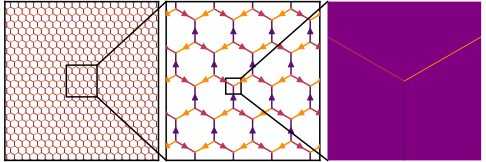
\includegraphics[width=\columnwidth]{figure_code/amk_chapter/honeycomb_zoom/intro_figure_template}
    \caption{\textbf{(a)} The standard Kitaev Model is defined on a honeycomb lattice. The special feature of the honeycomb lattice that makes the model solveable it is that each vertex is joined by exactly three bonds i.e the lattice is trivalent. One of three labels is assigned to each \textbf{(b)} We represent the antisymmetric gauge degree of freedom $u_{jk} = \pm 1$ with arrows that point in the direction $u_{jk} = +1$ \textbf{(c)} A visual analogy for The majorana transformation can be visualised as breaking each spin into}
    \label{fig:honeycomb_zoom}
\end{figure}

In order to actually solve the model we need to figure out how to leverage these conserved quantities. The trick is not so much a trick as an almost perfect consequence of the structure of the model and perhaps this was in fact how Kitaev first came up with it. We know that a single spin$-1/2$ can be represented by fermionic creation and annihilation operators $\sigma^{\pm} = 1/2(\sigma^x \pm \sigma^y)$ through a Jordan-Wigner transformation~\cite{}, this gives one fermion for each spin. In turn a fermion can be broken into two Majorana fermions $c_1 = 1/\sqrt{1}(f + f^\dagger)$ and $c_2 = i/\sqrt{1}(f - f^\dagger)$. If we double up the Hilbert space we get four Majoranas per spin: 

So how do we solve it? The trick is to replace each spin operator with 4 majorana operators (equivalent to two fermionic operators). 
 
The honeycomb lattice is bipartite, which means that it can be subdivided into two sub-lattices with only between sub-lattice couplings. It is also trivalent which means that each vertex connects to exactly three others. Finally, the edges of the lattice are three colourable, which means we can make an assignment (x,y,z) such that each site is connected to one of each type of edge. 

\subsection{Lattice generation}
% \begin{figure}
%     \centering
%     \includegraphics[width = \textwidth]{figs/pbc_voronoi.eps}
%     \caption{The construction of a periodic trivalent graph from a point set. The point set is replicated, a Voronoi transform is taken and finally the replication is undone. The graphs generated are trivalent except in very fine tuned cases which occur with low probability.}
%     \label{fig:pbc_voronoi}
% \end{figure}

We start from a set of points in the unit square. These can be drawn uniformly or via other methods such as using blue-noise or jammed circle packing. 

We then tile the plane with images of the point in the unit square and perform a voronisation over them. After this we can get rid of the images and relabel edges that cross the boundaries (red lines in fig \ref{fig:pbc_voronoi}) such that they connect points to the equivalent point within the unit cell.

We represent the graph structure with an ordered list of edges \((i,j)\) so we can represent both directed and undirected graphs which is useful for defining the sign of bond operators \(u_{ij} = - u_{ji}\).

% \subsetion{Kitaev-Heisenberg Model}
% In real materials there will generally be an addtional small Heisenberg term
% \begin{equation}
%     \label{eqn:kitaev_heisnberg}
%     \mathcal{H} =  - \sum_{\langle j,k\rangle_\alpha} J^{\alpha}\sigma_j^{\alpha}\sigma_k^{\alpha} + \sigma_j\sigma_k
% \end{equation}

% \section{The Projector} \label{apx:projector}
% {\color{red} Add brief mention of fermions and many body ground state}
% Closely following the derivation of~\cite{pedrocchiPhysicalSolutionsKitaev2011} we can extend to the amorphous case relatively simply. The main quantity needed is the product of the local projectors \(D_i\)
% \[\prod_i^{2N} D_i = \prod_i^{2N} b^x_i b^y_i b^z_i c_i \]
% for a lattice with \(2N\) vertices and \(3N\) edges. The operators can be ordered by bond type without utilising any property of the lattice.
% \[\prod_i^{2N} D_i = \prod_i^{2N} b^x_i \prod_i^{2N} b^y_i \prod_i^{2N} b^z_i \prod_i^{2N} c_i\]
% The product over \(c_i\) operators reduces to a determinant of the Q matrix and the fermion parity. The only problem is to compute the factors \(p_x,p_y,p_z = \pm1\) that arise from reordering the b operators such that pairs of vertices linked by the corresponding bonds are adjacent.
% \[\prod_i^{2N} b^\alpha_i = p_\alpha \prod_{(i,j)}b^\alpha_i b^\alpha_j\]
% This is simple the parity of the permutation from one ordering to the other and can be computed easily with a cycle decomposition.

% The final form is almost identical to the honeycomb case with the addition of the lattice structure factors \(p_x,p_y,p_z\)
% \[P^0 = 1 + p_x\;p_y\;p_z \mathrm{det}(Q^u) \; \hat{\pi} \; \prod_{\{i,j\}} -iu_{ij}\] 

% \(\mathrm{det}(Q^u)\) is the determinant of the matrix that takes \((c_1, c_2... c_{2N}) Q = (b_1, b_2... b_{2N})\). This along with \(\prod u_{ij}\) depend on the lattice and the particular vortex sector. 

% \(\hat{\pi} = \prod{i}^{N} (1 - 2\hat{n}_i)\) is the parity of the particular many body state determined by fermionic occupation numbers \(n_i\). The Hamiltonian is \(H = \sum \epsilon_i (n_i - 1/2)\) in this basis and this tells use that the ground state is either an empty system with all \(n_i = 0\) or a state with a single fermion in the lowest level. 



	        Conserved quantities -> plaquettes
			Majorana representation with 4 per site
			Alternative representation with with 3 majoranas per site
			Mapping to BdG hamiltonian
			Vortex defects and lattice defects
		    Kitaev on surfaces of genus g > 2

Plaquette Operators
Majorana representations
4 Majorana representation
3 Majorana representation
		    
\subsection{Amorphous Models}
			\subsection{The Weire-Thorpe Model}
			As a way to sanity check the code I was writing to work with the Kitaev Honeycomb Model on Amorphous lattices it was useful to reproduce some existing results. 
		
	

\section{The Amorphous Kitaev Honeycomb Model}
		Extending the kitaev honeycomb model to arbitrary trivalent lattices.
		Even and Odd Plaquettes
        Degeneracy and euler's equation

\begin{figure}
    \centering
    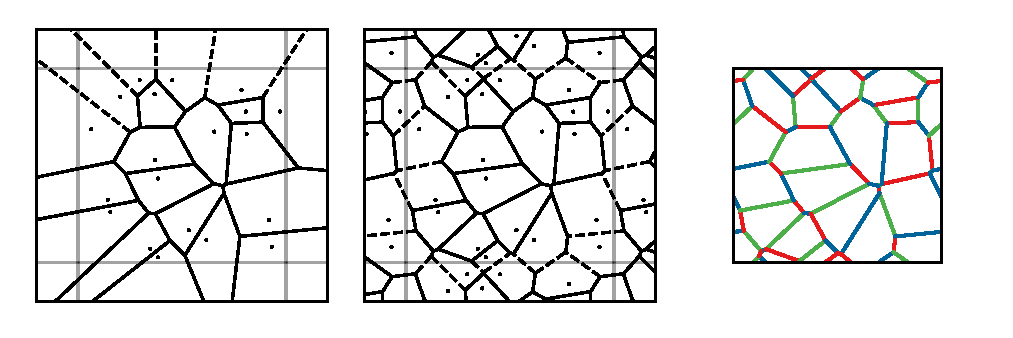
\includegraphics[width=\columnwidth]{figure_code/amk_chapter/lattice_construction/lattice_construction}
    \caption{\textbf{(a)} In-gap fermionic wavefunction drawn from the ground state flux sector in open boundary conditions, showing the state corresponds to a topological edge mode. Cut of the density along a line of lattice sites spanning the system (black line) is shown in the bottom subfigure on a logarithmic scale, demonstrating the characteristic exponential decay of topological edge modes with distance from the system edge. \textbf{(b)} Ground-state flux sector fermionic density of states in open boundary conditions, colored by inverse participation ratio. The increased inverse participation ratio of the in-gap states signifies their localisation to the edges of the system.}
    \label{fig:lattice_generation}
\end{figure}


\section{Methods}
        \subsection{Generating and Colouring Trivalent Graphs}
		\subsubsection{Voronisation}
		\subsubsection{Coloring}
		    The four colour theorem and its relation to edge colouring.
		    Finding Lattice colourings in practice: SAT solvers 
		
		\subsection{Finding the Ground State Flux Sector}
            A* star on the graph
		    Minimum spanning trees
    
\section{Results}
    \subsection{The Ground State}
	\section{Ground State Phase Diagram}
	\subsection{The Flux Gap}
	
		
\section{Conclusion}
\section{Discussion}
\section{Future Work}

\section{The Kitaev Honeycomb Model}

\subsection{The spin model}
The Kitaev-Honeycomb model is an exactly solveable model of interacting spins (or generic spin 1/2 degrees of freedom) on a honeycomb lattice. The Honeycomb lattice is bipartite and trivalent (each vertex connects to three others). The edges of the lattice are assigned to (x,y,z) such that each site is connected to one of each type of edge. 

\[H = \sum_{<i,j>} J_\alpha \sigma_i^{\alpha} \sigma_j^{\alpha} = \sum_{<i,j>} J_\alpha K_{ij}\]
where \(\alpha = \alpha(i,j)\) is the type of the bond linking sites i and j.

Various generalisations have been made, one mode replaces pairs of hexagons with heptagons and pentagons \cite{periNonAbelianChiralSpin2020} and another that replaces vertices of the hexagons with triangles \cite{yaoExactChiralSpin2007}. When we generalise this to the amorphous case, the key property that will remain is that each vertex interacts with exactly three others via an x, y and z edge. However the lattice will no longer be bipartite, breaking chiral symmetry among other things. 

The Hamiltonian commutes with the plaquette operators \(W_p\), products of the Ks around a plaquette. The Ks also commute with one another.
\[W_p = \prod_{<ij> \in P} K_{ij} = K_{12}K_{23}K_{34}K_{56} ... K_{N1}\]

Expanding the bond operators \(K_{ij} = \sigma_i^{\alpha} \sigma_j^{\alpha}\), Pauli operators on each site appear in adjacent pairs so can be replaced via \(\sigma_i \sigma_j = \delta_{ij} + \epsilon_{ijk} \sigma_k\) giving a product of Pauli matrices associated with the outward pointing bonds from the plaquette. In the general case:
\[W_p = \prod_{i \in P} i (-1)^{c_i} \sigma_i\]
where \(c_i = 0,1\) measures the handedness of the edges around vertex i, see Fig \ref{fig:handedness}. Plaquette operators for plaquettes with even numbers of edges square to 1 and hence have eigenvalues \(\pm 1\), while those around odd plaquettes have eigenvalues \(\pm i\) breaking chiral symmetry. The values of the plaquette operators partition the Hilbert space of the Hamiltonian into a set of flux sectors.


% \begin{figure}
%     \centering
%     \includegraphics[width = 0.5\textwidth]{figs/vertex_handedness}
%     \caption{Plaquette operators defined as a clockwise product of bond operators will contain a term \(...K_{ki}K_{ij}... = ...\sigma^\alpha_i \sigma^\beta_i ...\) which can be replaced with \(i (-1)^{c_i} \sigma_i^\gamma\) where \(c_i = 1\) if the bond types going clockwise around vertex i are a cyclic permutation of xyz otherwise \(c_i = 0\)}
%     \label{fig:handedness}
% \end{figure}

\subsection{A non-interacting Majorana representation}

The original Kitaev paper uses a transformation involving two fermionic modes per lattices site:
\[\acomm{f^\dagger}{f} = 1, \acomm{f}{f} = \acomm{f^\dagger}{f^\dagger} = 0\]
and the same for the second operator \(g\). They anti-commute with each other and the operators on other sites. It is also possible to transform to a Majorana basis with no redundant degrees of freedom \cite{fengTopologicalCharacterizationQuantum2007}.

We also have the number operators \(n_f = f^\dagger f\) and the total parity operator \(P = (2n_f - 1)(2n_g - 1)\) which divides the Hilbert space into even (\(\ket{00}, \ket{11}\)) and odd (\(\ket{01}, \ket{10}\)) parity subspaces. 

The Majorana modes are defined by:
\[b^x = f + f^\dagger\]
\[b^y = -i(f - f^\dagger)\]
\[b^z = g + g^\dagger\]
\[c = -i(g - g^\dagger)\]

Note that applying an odd number of Majorana operators to a state in one parity subspace will flip it to the other, while any even number preserves the parity subspace. 

The Pauli operators live in a two dimensional Hilbert space. We can build one from the fermionic subspace by projecting onto either the odd or even parity subspace defined above. The parity can be easily defined in terms of Majorana operators:

\[D = b^x b^y b^z c = - (2n_f - 1)(2n_g - 1) = - P\]

And the Pauli operators can be defined w.r.t states with D = 1 :
\[\sigma^\alpha = i b^\alpha c\]

With this choice, the Hamiltonian becomes quadratic:

\[H = \frac{i}{4} \sum_{<i,j>} 2 J_{\alpha_{ij}} u_{ij} c_i c_j\]
\[u_{ij} = i b^{\alpha_ij}_i b^{\alpha_ij}_j\]



\section{The Kitaev Honeycomb Model extended to an Amorphous Lattice}




\subsection{Edge Colouring}
% \begin{figure}
%     \centering
%     \includegraphics[width = .5\textwidth]{figs/dual_graphs.png}
%     \caption{Two graphs which are dual of one another.}
%     \label{fig:dual_graphs}
% \end{figure}

% \begin{figure}
%     \centering
%     \includegraphics[width = \textwidth]{figs/k5}
%     \caption{Embedings of the complete graph \(K_5\) and its dual \(D(K_5)\) onto the torus. The vertices of \(K_5\) cannot be 4 coloured and the edges of \(D(K_5)\) cannot be 3 coloured.}
%     \label{fig:k5}
% \end{figure}

Now that we have trivalent amorphous lattices, we need to assign \(\sigma_x, \sigma_y, \sigma_z\) to each edge. If we want the Majorana transformation to remain useful then we require that each site be connected to exactly on of each type of edge, otherwise the bond operators \(u_{ij}\) would not commute with one another and the model would not reduce to a quadratic form. This amounts to asking for a 3 coloring of the edges of the graph. 

The famous 4 colouring theorem proves that the vertices of all planar graphs can assigned one of four colors such that no neighbouring vertices share a colour using 4 colors or more. This can be turned into a proof that all trivalent planar graphs can be 3 edge coloured as follows:

1) Define the dual of a graph G to be D(G) such that plaquettes of G become vertices of D(G) and neighbouring plaquettes sharing an edge in D(G). It's easy to see that if G is planar then so is D(G). Note that each edge in G corresponds to an edge in D(G) and each vertex of G is surrounded by a triangle of three vertices in D(G).

2) The vertices of D(G) can be 4 coloured with colors (a,b,c,d)

3) Assign a color from (i,j,k) to the edges of D(G) (and thus to the edges of G) according to the colors of the vertices linked by the edge, ignoring ordering:

i if {a,b} or {c,d}
j if {a,c} or {b,d}
k if {a,d} or {b,c}

4) In a trivalent graph G, a vertex v in G is always part of 3 plaquettes (vertices in D(G)) and the colors of those plaquettes determines the colors of the edges that connect to v. The three vertices in D(G) must take three distinct colors from (a,b,c,d) so cannot lead to two edges with the same colour.

This implies that all trivalent planar graphs can have their edges 3 coloured. However we work in periodic boundary conditions and it's easy to embed the complete graph \(K_5\) into periodic boundary conditions, showing that the four colour theorem does not apply to periodic boundary conditions. However numerically we have not yet encountered even one case.

% \begin{figure}
%     \centering
%     \includegraphics[width = \textwidth]{figs/edge_color}
%     \caption{On the left, a single vertex in G, and the three dual-vertices in its dual D(G). If the dual-vertices of D(G) are 4 colored, the three dual-vertices shown must be three distinct colors, and hence if the colors of the edges in G are chosen according to the rules on the right, each will be distinct.}
%     \label{fig:edge_color}
% \end{figure}

\subsection{Finding Colourings}

Graph colouring is in NP, meaning that in general there is unlikely to be a polynomial time algorithm to compute it. However that does not mean that realistic instances of the problem are computationally intractable. A common method in computer science is to map NP problems onto a particular problem called Boolean Satisfiability for which general purpose and highly optimised solvers have been written.

The problems can be written as a a series of statements about a set of boolean variables, which we choose to be take to be the set \(l_{i\alpha}\) which indicate if edge i has colour \(\alpha\). We then have two types of contraint: each edge is exactly on colour and no neighbouring edges are the same color. 

I'll fill in the encoding later but the gist is that we can give this to a solver and get back: whether the problem is solveable, a solution or all the possible solutions. Finding a solution is relatively fast, while finding all the solutions is slower since there appear to be exponentially many of them. Fig \ref{fig:multiple_colourings} shows some examples. 


% \begin{figure}
%     \centering
%     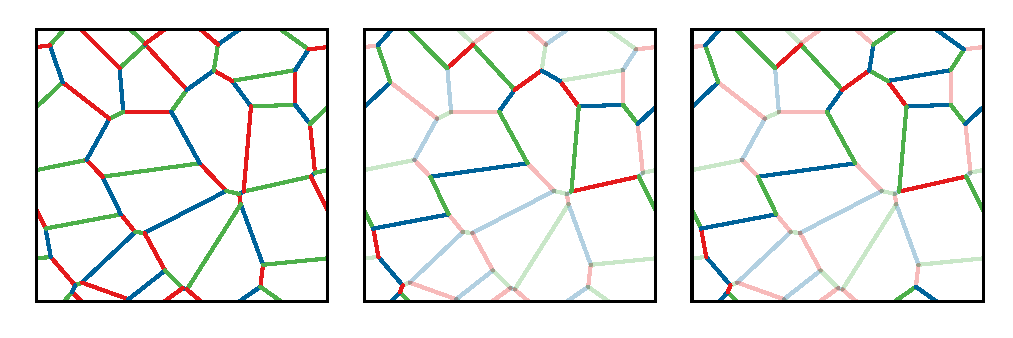
\includegraphics[width = \textwidth]{figs/multiple_colourings}
%     \caption{Multiple valid 3-edge-colourings of a random trivalent lattice. Edges are colored from red, green and blue and vertices are coloured red/blue if the edge colours are a cyclic/anticyclic permutation of rgb going clockwise around the vertex. Black edges or vertices indicate the color is the same as that in the top left. Note that some of the points are very close together, in future we will add a step to separate these.}
%     \label{fig:multiple_colourings}
% \end{figure}


\section{Weaire-Thorpe Models}
As a benchmark for our graph algorithms we reproduce results on the Weaire-Thorpe Model. The DOS agree very well but I haven't yet understood how to plot the edge states, plotting a single state in the gap or the sum of states in a finite energy region in the gap doesn't seem to look like an edge state.



% \begin{figure}
%     \centering
%     \includegraphics[width = \textwidth]{figs/WT_lattice}
%     \caption{An example of a Weaire-Thorpe model generated with our code.}
%     \label{fig:WT_lattice}
% \end{figure}

% \begin{figure}
%     \centering
%     \includegraphics[width = \textwidth]{figs/DOS_WT_Comp}
%     \caption{A comparison between the DOS from the paper (left) and the DOS generated using our code (right)}
%     \label{fig:DOS_WT_Comp}
% \end{figure}


\section{Open Questions}
\begin{itemize}
    \item Are the excitation spectra of the flux sectors disparate or overlapping?
    \item Will there be a qualitative difference between choosing +i for all plaquettes of odd length and of choosing +/-i so that they cancel out?
    \item
\end{itemize}

\section{The Projector}
Closely following the derivation given in~\cite{} we can extend the derivation of the projector to the amorphous case relatively simply. The final form is
\[P^0 = 1 + (-1)^{p_x + p_y + p_z} \left(-i \prod_{\{i,j\}} u_{ij}\right) \mathrm{det}(Q^u) \; \hat{\pi} \] 
where \(p_x,p_y,p_z\) are the parities of the permutations required to reorder the \(b^\alpha_i\) operators into an order where bonded sites are adjacent. These only depend on properties of the amorphous lattice used. In the HLM these terms can be computed analytically once a particular honeycomb lattice has been specified, we instead compute then numerically using a fast cycle decomposition algorithm.

\(\mathrm{det}(Q^u)\) is the determinant of the matrix that takes \((c_1, c_2... c_{2N}) Q = (b_1, b_2... b_{2N})\). This along with \(\prod u_{ij}\) depend on the lattice and the particular vortex sector. 

Finally \(\hat{\pi} = \prod{i}^{N} (1 - 2\hat{n}_i)\) is the parity of the particular many body state determined by fermionic occupation numbers \(n_i\). The Hamiltonian is \(H = \sum \epsilon_i (n_i - 1/2)\) in this basis and this tells use that the ground state is either an empty system with all \(n_i = 0\) or a state with a single fermion in the lowest level. 

\subsection{Derivation}
The projector is just a product of the site projectors, let's say there are \(2N\) sites.
\[D_i = b^x_i b^y_i b^z_i c_i \]
\[P = \prod_i^{2N} (1 + D_i)\]

The clever trick from \ref{} is to note that this corresponds to a sum over products of all possible subsets of the integers (the powerset) of our 2N \(D_i\) operators. 

If we think of these subsets as bitstrings of length \(2N\) the we can write this as a sum over integers \(n\) where \(n_i = 0,1\) is the ith bit of \(n\).
\[P = \sum_{n = 0}^{2^{2N}} \prod_{i=0}^{2N} D_i^{n_i}\]

then the ``all ones'' operator \(F = \prod_i D_i\) acts as the bitwise not operation on any other subset:
\[ \prod_i D_i \prod_{i=0}^{2N} D_i^{n_i} = \prod_{i=0}^{2N} D_i^{1 - n_i}\]
Hence we can actually just sum over half the integers and use this operator to get the other half:
\[P = \left(\sum_{n = 0}^{2^{2N - 1}} \prod_{i=0}^{2N} D_i^{n_i} \right) (1 + \prod_{i=0}^{2N} D_i) = S P^0\]

The paper argues that S will never give zero on any state for reasons I do not understand, though one can make an argument that since \(P^0\) already removes half the states from the Hilbert space, S cannot remove anymore.  We therefore focus on computing \(P^0\).

\[\prod_{i=1}^{2N} D_i = b^x_1 b^y_1 b^z_1 c_1\; b^x_2 b^y_2 b^z_2 c_2\; ... \;b^x_{2N} b^y_{2N} b^z_{2N} c_{2N}\]

We can move all the \(c_i\) operators to the right, incurring \(3(i-1)\) swaps for each giving a factor of \(-1 ^ \theta_c\) where \( \theta_c = {3N(2N-1)} = \sum{i = 1}^{2N} 3(i-1)\)

\[\prod_{i=1}^{2N} D_i = -1^{\theta_c}b^x_1 b^y_1 b^z_1\; b^x_2 b^y_2 b^z_2\; ... \;b^x_{2N} b^y_{2N} b^z_{2N}\;\prod_{i=1}^{2N}c_i\]

All the \(b^x\) terms are separated by pair other operators so can be brought to the front with no additional factors.

\[\prod_{i=1}^{2N} D_i = -1^{\theta_c}\left(\prod_{i=1}^{2N}b^x_i\right) b^y_1 b^z_1\; b^y_2 b^z_2\; ... \; b^y_{2N} b^z_{2N}\;\left(\prod_{i=1}^{2N}c_i\right)\]

Finally we can send each \(b^z_i\) to the right incurring \(i\) swaps giving \(\theta_z = N(2N - 1)\) 

How to do open boundary conditions

Note: we don't actually compute \(p_x\) we compute \(-1ˆp_x\) directly using a cycle decomposition to compute the permutation parity.


    
    
    

% \chapter{Conclusion \& Discussion}
% \label{ch:conclusion}
%     % \section{Summary of Thesis Achievements}

\section{Discussion}


\section{Overall Conclusion}

% Applications.


\section{Future Work}

% Future Work.

% \appendix
%     % 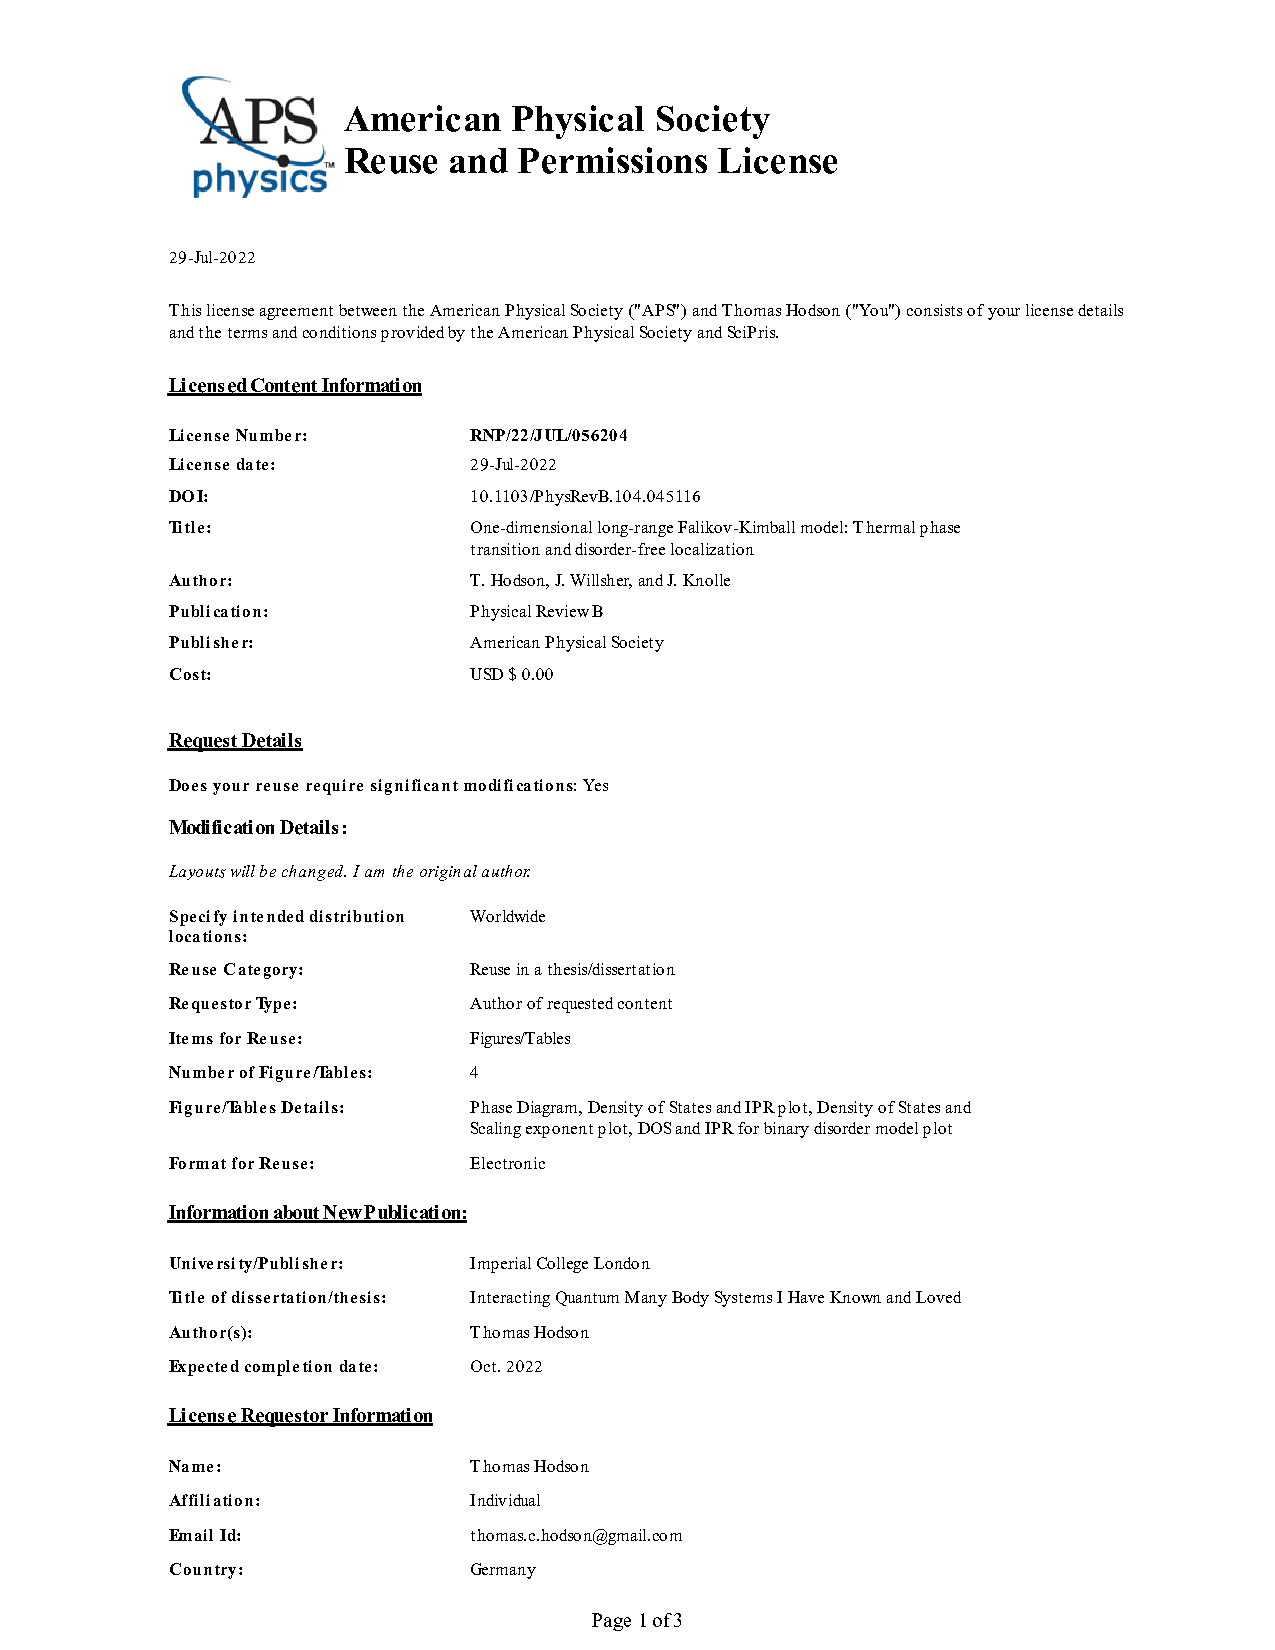
\includepdf[pages=-]{APS_copyright_permission.pdf}

\addcontentsline{toc}{chapter}{Bibliography}
\bibliographystyle{unsrt}
\bibliography{entire_zotero_library}

\end{document}